\documentclass{article}

\usepackage{forest}
\usetikzlibrary[intersections]
\usetikzlibrary[decorations.pathreplacing]
\usepackage{graphicx}
\usepackage{html}

\begin{document}

I am offerring GNU/Linux tutoring to those who may be interested.  See \strikeout{this flyer} (not currently advertising) for details.  Here are some cool examples below:

% Minetest example
\section{Minetest}
Minetest is a voxel game engine (and game) like Minecraft, except that Minetest is Free Software, thus you have the right to modify the code and redistribute copies to your friends and family.

The game world itself is generated using \htmladdnormallink{Perlin Noise}{https://en.wikipedia.org/wiki/Perlin\_noise}.  Modifying the noise parameters can result in some very interesting maps.  For example, dramatically increasing the size of caves results in:
\begin{center}
\includegraphics[scale=0.25]{files/minetest_mapgen.png}
\end{center}
It is also possible to create mountains thousands of blocks tall, or large rivers with only a few pockets of land in-between them.

The most powerful aspect of Minetest is its modding API (Application Programming Interface).  This allows virtually unlimited customization of the game.  A simple example is the \texttt{farming\_plus} mod, which adds extra farmable plants, trees, and a scarecrow:
\begin{center}
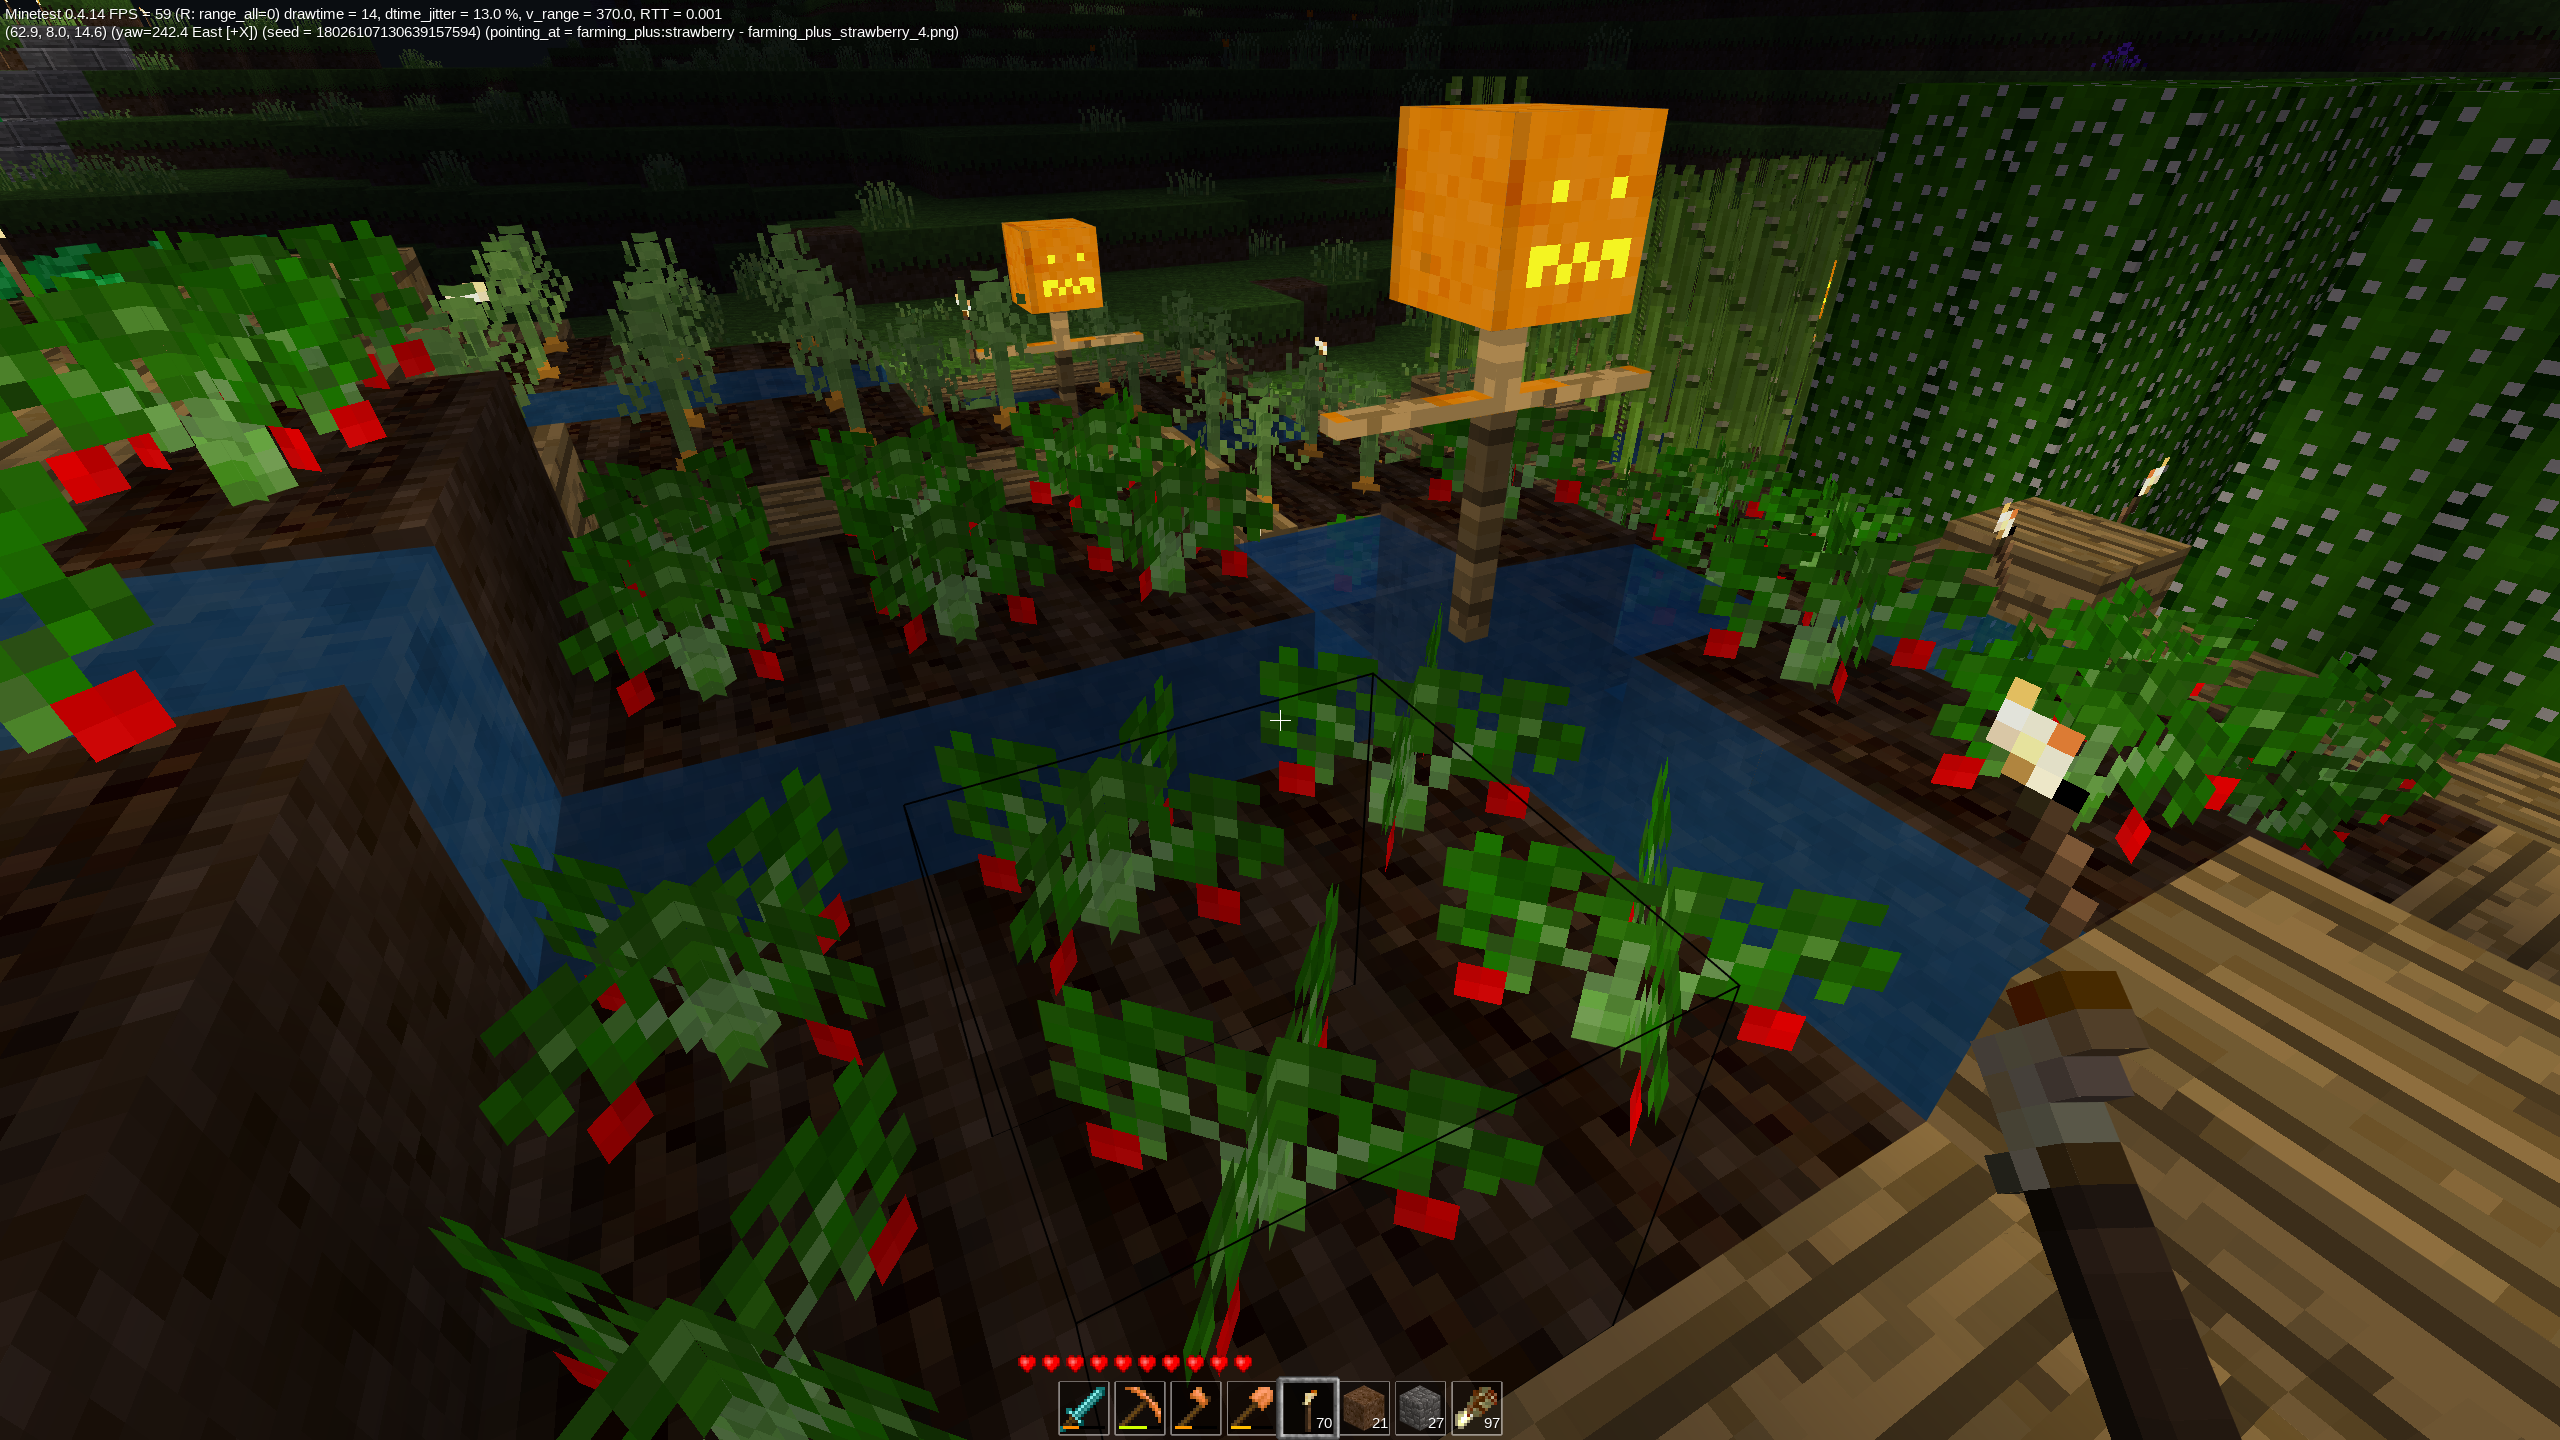
\includegraphics[scale=0.25]{files/minetest_farming.png}
\end{center}
I modified the strawberry plant textures to make them look more like strawberry plants, although I was told that it now somewhat resembles broccoli.

Learning Minetest is a great way to play, code, and share freely!

% LaTeX example
\section{\LaTeX}
\LaTeX is a document-preparation system, like that \emph{other} word-processor, but far superior for complex documents and mathematical typesetting.  This is an example of a recursion tree which I typeset in \LaTeX:
\begin{center}
\begin{makeimage}
\reflectbox{\reflectbox{% _THIS_ exists because otherwise LaTeX2HTML can't figure out where and how to crop the damn image.
\begin{forest}
[$n$, for tree={s sep=-1mm},name=level1
	[1/2
		[1/4,for descendants={edge=dotted}
			[]
			[]
			[]
		]
		[1/4,for descendants={edge=dotted}
			[]
			[]
			[]
		]
		[1/4,for descendants={edge=dotted}
			[]
			[]
			[]
		]
	]
	[1/2
		[1/4,for descendants={edge=dotted}
			[]
			[]
			[]
		]
		[1/4,for descendants={edge=dotted}
			[]
			[]
			[]
		]
		[1/4,for descendants={edge=dotted}
			[]
			[]
			[]
		]
	]
	[1/2,name=level2
		[1/4,for descendants={edge=dotted}
			[]
			[]
			[]
		]
		[1/4,for descendants={edge=dotted}
			[]
			[]
			[]
		]
		[1/4,for descendants={edge=dotted},name=level3
			[]
			[]
			[,name=level4]
		]
	]
]
% Bottom leaves.
\node(bottombox) at ($(current bounding box.south) - (0, 1)$){};
\foreach \x in {-3, -2, ..., 0, 2, 3} {
	\node(leaf\x) at ($(bottombox.west) + (\x, 0)$){$T(1)$};
	\draw[dotted] (leaf\x) -- +(0, 1);
}
\node at ($(bottombox.west) + (1, 0)$){\ldots};
% Left side arrow thingy.
\node(leftbox) at ($(current bounding box.west) - (0.75, 0)$){$log_2(n)$};
\path (current bounding box.north west) -- (current bounding box.north) node(topline){};
\draw[->] (leftbox) -- (leftbox |- topline);
\path (current bounding box.south west) -- (current bounding box.south) node(botline){};
\draw[->] (leftbox) -- (leftbox |- botline);
% Right side sums.
\path ($(current bounding box.north east) + (0.5, 0)$) -- ($(current bounding box.south east) + (0.5, 0)$) node(rightline){};
\draw[-stealth,dotted,thick] (level1) -- (level1 -| rightline) node(l1node){};
\node at ($(l1node) + (1, 0)$){$n$};
\draw[-stealth,dotted,thick] (level2) -- (level2 -| rightline) node(l2node){};
\node at ($(l2node) + (1, 0)$){$\frac{3}{2}n$};
\draw[-stealth,dotted,thick] (level3) -- (level3 -| rightline) node(l3node){};
\node at ($(l3node) + (1, 0)$){$\frac{9}{4}n$};
\path[] (level4) -- (level4 -| rightline) node(l4node){};
\node at ($(l4node) + (1, 0)$){\vdots};
\draw[-stealth,dotted,thick] (leaf3) -- (leaf3 -| rightline) node(leafnode){};
\node (rightleaftotal) at ($(leafnode) + (1, 0)$){$\Theta n^{\log_2 3}$};
% Bottom brace.
\draw [decorate,decoration={brace,mirror}] (leaf-3.south west) -- (leaf3.south east) node(leaftotal)[midway,below]{$n^{\log_2(3)}$};
\end{forest}
}}
\end{makeimage}
\end{center}
\ldots this is the algorithmic complexity approximation derived from the recurrence tree:
\begin{center}
\begin{makeimage} % Also shouldn't be needed but otherwise it inserts lots of whitespace below the equation.
\begin{eqnarray*}
	T(n) &=& n + \frac{3}{2}n + \left(\frac{3}{2}\right)^2n + \cdots + \left(\frac{3}{2}\right)^{\log_2(n) - 1}n + \Theta(n^{\log_2(3)}) \\
	&=& \sum_{i=0}^{\log_2(n)-1} \left(\frac{3}{2}\right)^in + \Theta(n^{\log_2(3)}) \\
	&=& \frac{\left(\frac{3}{2}\right)^{\log_2(n)} - 1}{\left(\frac{3}{2}\right) - 1}n + \Theta(n^{\log_2(3)}) \\
	&=& (2(3/2)^{\log_2(n)} - 2)n + \Theta(n^{\log_2(3)}) \\
	&=& (2(n)^{\log_2(3/2)} - 2)n + \Theta(n^{\log_2(3)}) \\
	&=& (2(n)^{\log_2(3) - 1} - 2)n + \Theta(n^{\log_2(3)}) \\
	&=& 2n(n)^{\log_2(3) - 1} - 2n + \Theta(n^{\log_2(3)}) \\
	&=& 2n^{\log_2(3)} - 2n + \Theta(n^{\log_2(3)}) \\
	&=& \Theta(n^{\log_2(3)})
\end{eqnarray*}
\end{makeimage}
\end{center}
\ldots but this is just eye candy (or perhaps horrors from the abyss if you find math intimidating), what I cannot show you here is how much easier it is to construct references, tables of contents, indices, \&c.

% GPG example
\section{GNU Privacy Guard (GPG)}
The firearms of cyberspace: cryptography.  GPG is a software tool which allows users to make use of crytpography and send secure, encrypted messages to each other, thus protecting against eavesdropping.  Below is an example of a message encrypted with the password "password", which I can teach you how to decrypt:
\begin{verbatim}
-----BEGIN PGP MESSAGE-----

jA0EBwMCoA8RdMu6/AXC0nEBvudCVg9Sx/ErwvpK9C3OHj3bFKNy9Hg41eBFcZyg
ayyCB6lp6T5T4snj14j6qS89Rrqh3ljdrtXGRbviSH9Xoje6UrqC9Q6ejDDOuOFv
rxisUgkpCDWl4D494awiYuuksA34zMyfTQ13mPyx7Zodbg==
=/Lg2
-----END PGP MESSAGE-----
\end{verbatim}
Note that because the password is published here (and it is a weak password), this particular message is not actually secure.

\section{Algorithims}
\htmladdnormallink{This}{mergesort.ps} is a visualization of a 1,000-element \htmladdnormallink{Merge Sort}{https://en.wikipedia.org/wiki/Merge\_sort} which I generated using \texttt{graphviz}.  Note how the elements go from unsorted at the top to sorted at the bottom.  WARNING: This is a large image and may crash unstable image viewers or systems with little RAM.

\end{document}
